%! Author = Jonathan
%! Date = 2022-09-26

% Preamble
\documentclass[11pt]{article}
%check
% Packages
\usepackage[letterpaper, margin=1in]{geometry}
\usepackage[page,toc,titletoc,title]{appendix}
\usepackage{amsmath}
\usepackage{enumitem}
\usepackage{tabularx}
\usepackage{graphicx}
\usepackage{blindtext}
\usepackage{titlesec}
\usepackage{hyperref}
\usepackage{longtable}
\usepackage{mathrsfs}
\usepackage{amssymb}
\usepackage{marvosym} % additional math symbols
\usepackage[table, dvipsnames]{xcolor}
\definecolor{hyperColor}{RGB}{5, 99, 183}

\hypersetup{
    colorlinks=true,
    linkcolor={hyperColor},
    citecolor={blue!50!black},
    urlcolor={hyperColor}
}

\usepackage{tocloft} % Control table of contents, figures, etc
\renewcommand{\cftsecleader}{\cftdotfill{\cftdotsep}}
\providecolors{dvipsnames*}
\usepackage{wrapfig}
\usepackage{amsfonts} %TeX fonts from the American Mathematical Society
\usepackage[usenames,dvipsnames]{color}
\usepackage{stmaryrd}
\usepackage{booktabs}
\usepackage{float}
\usepackage{floatrow}
\usepackage[clean]{svg}
\usepackage{pdfpages}
\usepackage{parskip} % normal paragraph structure

\usepackage{titling}

\usepackage{biblatex}
\usepackage[english]{babel}
\usepackage[square,numbers]{natbib}
\usepackage{ulem}



\author{Alexander, Yonatan\\
\texttt{SN: 251097927}
\and
Aziz, Mohammad Yasin\\
\texttt{SN: 251282726}
\and
Kien Tang Tran, Michael\\
\texttt{SN: 250735158}
}
\title{Therapy Support App\\
\large Group 9}


% Document
\begin{document}


    \begin{titlepage}
        \begin{center}

            \phantom{.\\}
            \vspace{1cm}

            \begin{Huge}
                \textbf{My Mental Health App}
            \end{Huge}


            \vfill

            \begin{Large}
                \textbf{Group 9}\\
            \end{Large}

            \vspace{10pt}

            \begin{table*}[h]
                \centering
                \begin{tabular}{lrr}
                    \textbf{Alexander, Yonatan}      & \textbf{SN: 251097927} \\
                    \textbf{Kien Tang Tran, Michael} & \textbf{SN: 250735158} \\
                    \textbf{Aziz, Mohammad Yasin}    & \textbf{SN: 251282726} \\
                \end{tabular}
            \end{table*}


%            \textbf{
%                Alexander, Yonatan          (SN: 251097927)   \\
%                Kien Tang Tran, Michael       (SN: 250735158)                \\
%                Aziz, Mohammad Yasin     (SN: 251282726)}

            \vfill

            
\includegraphics[width=0.4\textwidth]{NewLogoEPS}   % App Logo


            \vfill


            Computer Science 4470A\\
            \textsl{The Department of Computer Science\\
            The University of Western Ontario}

            \vspace{5pt}
            \includegraphics[width=0.1\textwidth]{Stacked_CMYK}   % Western Logo
            \vspace{5pt}

            \today\\
            \textbf{Please do NOT post our group's video to the course's YouTube Channel.}

        \end{center}
    \end{titlepage}


%
%
%    \begin{enumerate}
%        \item Business requirements related to problem's root cause
%        \item Examples:
%        \begin{enumerate}
%            \item Accurate monthly sales forecast which will help us increase our sales
%            \item need to generate monthly report that indicates sales
%            \item notifications to account executives when a customer opens a problem ticket
%        \end{enumerate}
%        \item Varies based on process model
%        \item Expected:
%        \begin{enumerate}
%            \item Shippable product
%            \item some documentation
%            \item lessons learned
%            \item Why we chose one thing and not another
%            \item If we switched from one platform to another (if we switched)
%        \end{enumerate}
%        \item stakeholders:
%        \begin{enumerate}
%            \item identify asap
%            \item anyone who has any relation to the project
%            \item external - anyone who has an influence\; including people who write certain libraries and so on  (include instructor and TA as external stakeholders)
%            \item internal - programmers, maintainable, customers, users, etc [double check this point's list]
%        \end{enumerate}
%        \item success/acceptance criteria:
%        \begin{enumerate}
%            \item measurable terms of the project's outcome for the end user, customer, stakeholders, etc.
%            \item cost
%            \item timeline
%            \item Business requirements
%            \item scope
%            \item acceptance criteria: (can be only a few)
%            \begin{enumerate}
%                \item conditions the software must fulfill
%            \end{enumerate}
%        \end{enumerate}
%    \end{enumerate}


%    \maketitle
%    Cover sheet {Project title, Group members' names and SID}

    \pagebreak

    \tableofcontents

    \listoffigures

    \listoftables

    \pagebreak


    \section{Problem Definition}\label{sec:problem-definition}
    Therapists and patients encounter many small yet persistent challenges during the therapeutic process concerning the patients' ability to self-manage between sessions.

    While this project`s scope is not large enough to address them all, the following stood out to us:

    \begin{itemize}
        \item Mood tracking between sessions.
        \begin{itemize}
            \item Usually, at the start of a session therapists ask for an update about the time since the last session.
            However, self-reporting bias usually means that if the patient is having a bad day or is in a bad mood, their view on the time since the last session is skewed, sometimes heavily.
            Further, memory can be corrupted and events can easily be forgotten.
%            \begin{itemize}
%                \item numerical (including descriptions of the numeric values, to increase clarity)
%                \item statistical (based on numerical inputs)
%                \item descriptive (``gloomy``, ``sad``, etc)
%            \end{itemize}
        \end{itemize}
        \item Medication management
        \begin{itemize}
            \item Inventory (to not run out of important medications, mood stabilizers are a good example in the context of mental health especially)
            \item Persistence (taking medications as required and without missing a day)
        \end{itemize}
        \item Symptoms
        \begin{itemize}
            \item Medical (unrelated to the patients diagnosed )
        \end{itemize}
        \item Other self care aspects, such as sleeping, eating, etc.
    \end{itemize}
%
%    \begin{enumerate}
%        \item mood tracking between sessions
%        \begin{enumerate}
%            \item numerical (including descriptions of the numeric values, to increase clarity)
%            \item statistical (based on numerical inputs)
%            \item descriptive (``gloomy``, ``sad``, etc)
%        \end{enumerate}
%        \item Medication management
%        \begin{itemize}
%            \item Inventory
%            \item Persistence (taking medications as required)
%        \end{itemize}
%        \item Symptoms
%        \begin{itemize}
%            \item Medical (unrelated to the patients diagnosed )
%        \end{itemize}
%    \end{enumerate}


    \section{Project Objective}\label{sec:project-objective}

    \begin{enumerate}[label=O\arabic*]
%        \item User can add new entries, view existing entries, delete (remove) existing entries, to:
%        \begin{enumerate}
%            \item Mood.
%            \item Medications.
%            \item Symptoms.
%        \end{enumerate}
%        \item User will be able to view the entries from the past week, at a glance, in a dedicated view.
%        \item User can update new entries to:
%        \item The system will keep track of past entries.
%        \item Patients should be able to generate a report about their mood and medication for their therapy session in one to three clicks between each therapy session.
%        Therapists should be able to see their patient's mood and medication reports in one to two clicks between each therapy session.
        \item Patients can add new entries.
        \item Patients can view existing entries.
        \item Patients can delete existing entries.
        \item User will be able to view the entries from the past week, at a glance, in a dedicated view.
        \item Learning the process of project development through application of knowledge acquired during the Computer Science 4471A Course.
        \item The creation of an intuitive and user friendly self-management mobile app (Android ). %and/or i/OS
    \end{enumerate}
    \pagebreak


    \section{Stakeholders List}\label{sec:stakeholders-list}
    \begin{itemize}
        \item Patients - Internal stakeholder
    \end{itemize}

    \subsection{Internal Stakeholders}\label{subsec:internal-stakeholders}
    \item Therapists - External stakeholder
    \item external - anyone who has an influence\; including people who write certain libraries and so on  (include instructor and TA as external stakeholders)
    \item internal - programmers, maintainable, customers, users, etc [double check this point's list]

    \begin{enumerate}
        \item Patients (main users and the target audience).
    \end{enumerate}

    \subsection{External Stakeholders}\label{subsec:external-stakeholders}

    \begin{enumerate}
        \item Therapists
        \item Legislation and public policy (for example security of medical information)
        \item Governing bodies (such as the CRPO - The College of Registered Psychotherapists of Ontario)
        \item Instructor
        \item TA
        \item Libraries:
        \begin{enumerate}
            \item Android.
            \item Google.
            \item MPAndroid (to create the graphs).
            \item JetBrains (makers of Android Studio).
            \item Java Libraries
        \end{enumerate}
    \end{enumerate}

    \pagebreak


    \section{Success/Acceptance Criteria for each Stakeholder}\label{sec:success/acceptance-criteria-for-each-stakeholder}


    \begin{itemize}
        \item As a user, I want to be able to store my mood on a particular day, on a scale of 0 to 10.
        \item As a user, I want to be able to store my medication details such as the medication, dosage, etc.
        \item As a user, I want to be able to store my symptom details on a particular day.
        \item As a user, I want to be able to view my past mood reports for my therapy visit.
        \item As a user, I want to be able to view my past symptoms for my therapy visit.
        \item As a user, I want to be able to view my past medications for my therapy visit.
    \end{itemize}

    \pagebreak


    \section{Use case diagram(s)}\label{sec:use-case-diagram(s)}

    \subsection{Use case Diagram 1: Mood}\label{subsec:use-case-diagram-1:-Mood}
    \begin{figure}[H]
        \centering
        \includegraphics[height=0.3\textheight]{Diagrams/Use Case Diagrams/Use Case Diagram 1}
        \caption{Use case Diagram 1: The Mood Subsystem}
        \label{fig:Use case Diagram 1: The Mood Subsystem}
    \end{figure}

    Contains the Mood subsystem.

    \subsection{Use case Diagram 2: Medication}\label{subsec:use-case-diagram-2:-medication}
    \begin{figure}[H]
        \centering
        \includegraphics[height=0.3\textheight]{Diagrams/Use Case Diagrams/Use Case Diagram 2}
        \caption{Use case Diagram 2: The Medication Subsystem}
        \label{fig:Use case Diagram 2: The Medication Subsystem}
    \end{figure}

    Contains the Medication subsystem.

    \subsection{Use case Diagram 3: Symptom}\label{subsec:use-case-diagram-3:-Symptom}
    \begin{figure}[H]
        \centering
        \includegraphics[height=0.3\textheight]{Diagrams/Use Case Diagrams/Use Case Diagram 3}
        \caption{Use case Diagram 3: The Symptom Subsystem}
        \label{fig:Use case Diagram 3: The Symptom Subsystem}
    \end{figure}

    Contains the Symptom subsystem.

    \pagebreak


    \section{Use case Descriptions}\label{sec:use-case-descriptions}

    \subsection{Use case Description: Add Medication}\label{subsec:use-case-description:-add-medication}

    \textbf{Use Case Name:} Add Medication\\
    \textbf{Scenario:} Add medication entry to database.\\
    \textbf{Brief Description:} When a Patient (User) enters information for a new medication entry and presses ``Submit'', add the information to the medications' table in the database.\\
    \textbf{Triggering Event:} Patient (User) enters the ``Medication'' view.\\
    \textbf{Actors:} Patient (User)\\
    \textbf{Related Use cases:} Update Medication, Delete Medication, Browse Medication History\\
    \textbf{Stakeholders:} Patient\\
    \textbf{Preconditions:} App is open on the ``Medications'' Screen.\\
    \textbf{PostConditions:} A new entry was added to the medications' table in the database.\\
    \textbf{Flow of Activities:}

    \begin{table}[H]
        \begin{tabularx}{\textwidth} {
            | >{\raggedright\arraybackslash}X
            | >{\raggedright\arraybackslash}X |  }
            \toprule
            \textbf{Actor}                                                            & \textbf{System}                                \\
            \midrule
            1. User opens ``Medications'' screen                                      &                                                \\
            \hline
            2. User fills the ``Enter the medication name'' field                     &                                                \\
            \hline
            3. (Optional) User fills the ``Enter the brand name'' field               &                                                \\
            \hline

            4. (Optional) User fills the ``Enter the medication quantity'' field      &                                                \\
            \hline

            5. (Optional) User fills the ``Enter the medication quantity unit'' field &                                                \\
            \hline

            6. (Optional) User fills the ``Enter the medication frequency'' field     &                                                \\
            \hline

            7. User pressed ``Add Medication Entry''                                  & 7.1 System confirms step 2 was completed       \\
            \phantom{0}                                                               & 7.2 System updates the database with new entry \\
            \bottomrule
        \end{tabularx}
        \caption{Use case Description: Add Medication, Flow of Activities}\label{tab:table2}
    \end{table}

    \textbf{Exception conditions:}

    The user did not fulfill step 2.

    \subsection{Use case Description: Browse Medication History}\label{subsec:use-case-description:-browse-medication-history}

    \textbf{Use Case Name:} Browse Medication History\\
    \textbf{Scenario:} The user wants to view the medication entries.\\
    \textbf{Brief Description:} When a Patient (User) enters opens the ``Medication List'' view, the list of medications should appear.\\
    \textbf{Triggering Event:} Patient (User) enters the ``Medication List'' view.\\
    \textbf{Actors:} Patient (User)\\
    \textbf{Related Use cases:} Update Medication, Delete Medication, Add Medication\\
    \textbf{Stakeholders:} Patient\\
    \textbf{Preconditions:} App is open on any non-``Medications List'' Screen.\\
    \textbf{PostConditions:} None (can be empty).\\
    \textbf{Flow of Activities:}

    \begin{table}[H]
        \begin{tabularx}{\textwidth} {
            | >{\raggedright\arraybackslash}X
            | >{\raggedright\arraybackslash}X |  }
            \toprule
            \textbf{Actor}                               & \textbf{System}                                                          \\
            \midrule
            1. User opens the ``Medication List'' screen & 1.1 The system propagates past entries into the view (if there are any). \\
            \bottomrule
        \end{tabularx}
        \caption{Use case Description: Browse Medication History, Flow of Activities}\label{tab:table3}
    \end{table}

    \pagebreak


    \section{Sequence diagram(s) {for the selected use case for descriptions}}\label{sec:sequence-diagram(s)}

    \subsection{Sequence Diagram 1: Add Medication}\label{subsec:sequence-diagram-1:-add-medication}
    \begin{figure}[H]
        \centering
        \includegraphics[width=\textwidth]{Diagrams/Use Case Diagrams/Sequence diagram 1}
        \caption{Class Diagram: Relationships.}
        \label{fig:Sequence Diagram 1: Add Medication}
    \end{figure}

    \subsection{Sequence Diagram 2: Browse Medication History}\label{subsec:sequence-diagram-2:-browse-medication-history}
    \begin{figure}[H]
        \centering
        \includegraphics[width=\textwidth]{Diagrams/Use Case Diagrams/Sequence diagram 2}
        \caption{Class Diagram: Relationships.}
        \label{fig:Sequence Diagram 2: Browse Medication History}
    \end{figure}


    \pagebreak


    \section{System Architecture}\label{sec:system-architecture}

    Unfortunately, writing the code in Java meant that our chosen architecture (Model-View-ViewModel) was not feasible, resulting in needing to change the System Architecture to Model View Controller very late in development.

    \textbf{System Architecture: Model View Controller}.

    \pagebreak


    \section{Detailed Class diagram(s)}\label{sec:detailed-class-diagram(s)}

    \begin{figure}[H]
        \centering
        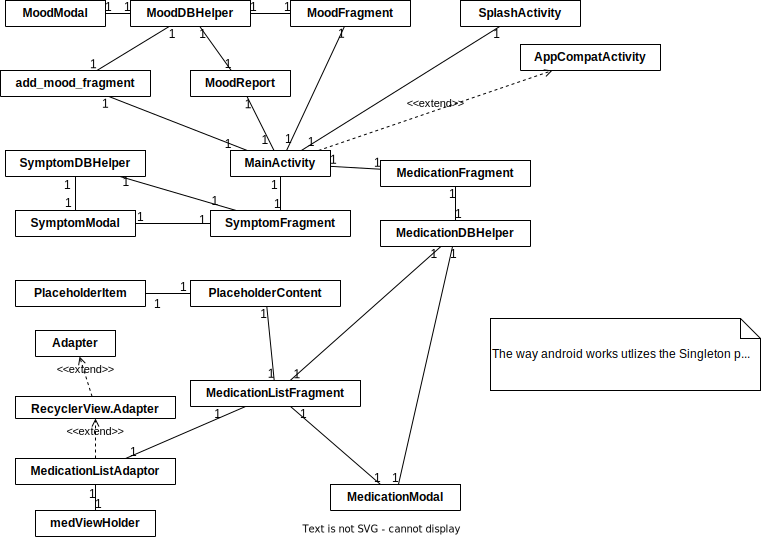
\includegraphics[width=\textwidth]{Diagrams/Class Diagrams/Class Diagram-Class Relationships (No Method)}
        \caption{Class Diagram: Relationships.}
        \label{fig:figure}
    \end{figure}

    Contains \textbf{all} classes in the system, and the relationships between them.
    The other class diagrams contain the respective methods.

    \begin{figure}[H]
        \centering
        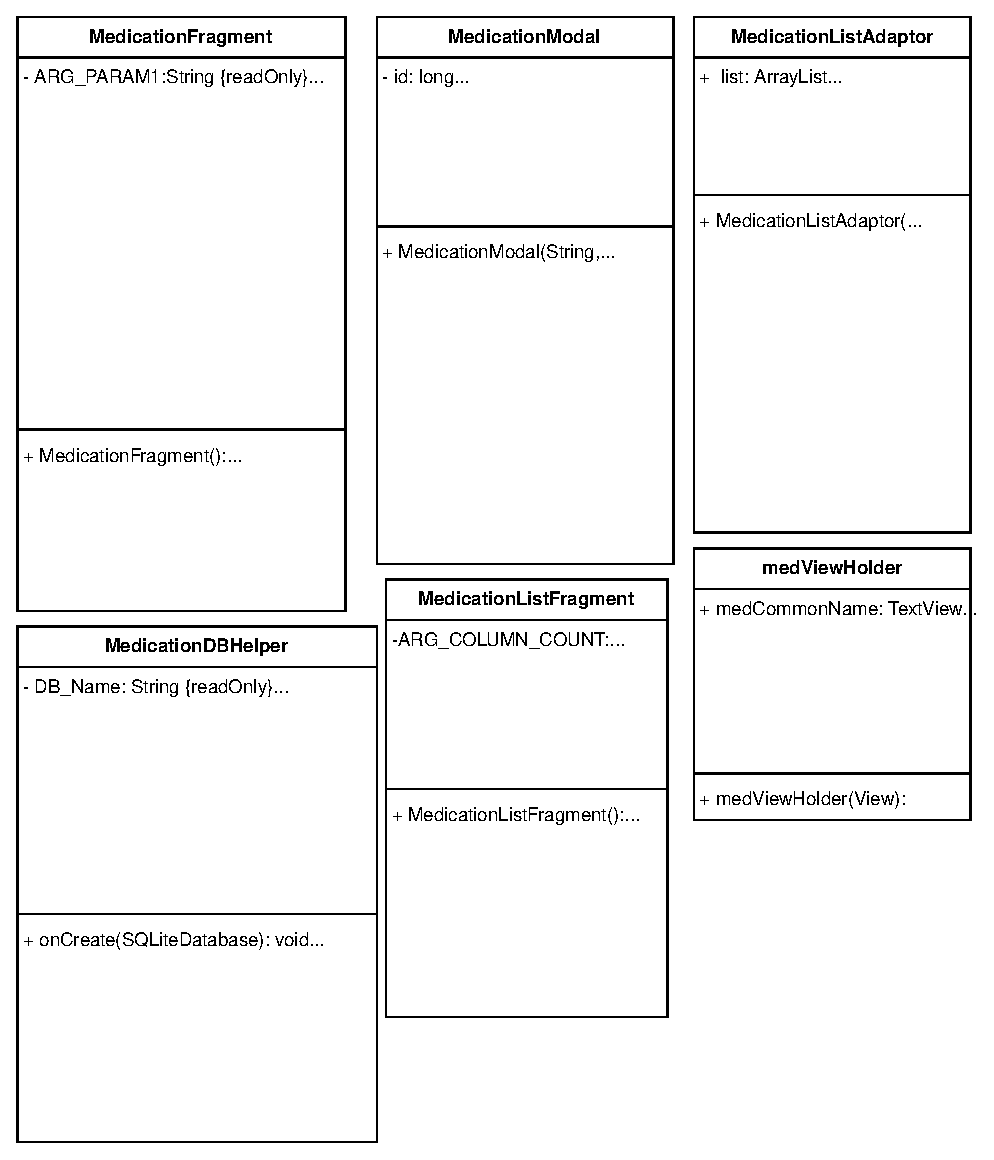
\includegraphics[width=\textwidth]{Diagrams/Class Diagrams/Class Diagram-Medication Classes}
        \caption{Class Diagram: Medication}
        \label{fig:figure1}
    \end{figure}

    Contains \textbf{all} classes relating directly Medications.
    Relationships included only as part of \textit{Class Diagram: Medication}.

    \begin{figure}[H]
        \centering
        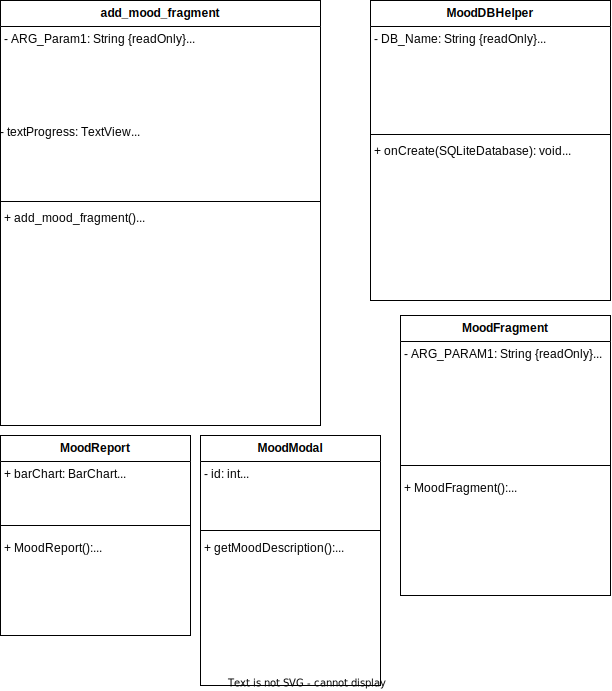
\includegraphics[width=\textwidth]{Diagrams/Class Diagrams/Class Diagram-Mood Classes}
        \caption{Class Diagram: Mood}
        \label{fig:figure2}
    \end{figure}

    Contains \textbf{all} classes relating directly Mood.
    Relationships included only as part of \textit{Class Diagram: Medication}.

    \begin{figure}[H]
        \centering
        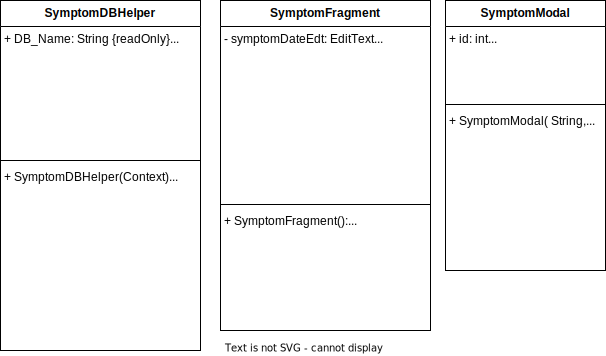
\includegraphics[width=\textwidth]{Diagrams/Class Diagrams/Class Diagram-Symptoms Classes}
        \caption{Class Diagram: Symptoms}
        \label{fig:figure3}
    \end{figure}

    Contains \textbf{all} classes relating directly Symptoms.
    Relationships included only as part of \textit{Class Diagram: Medication}.

    \begin{figure}[H]
        \centering
        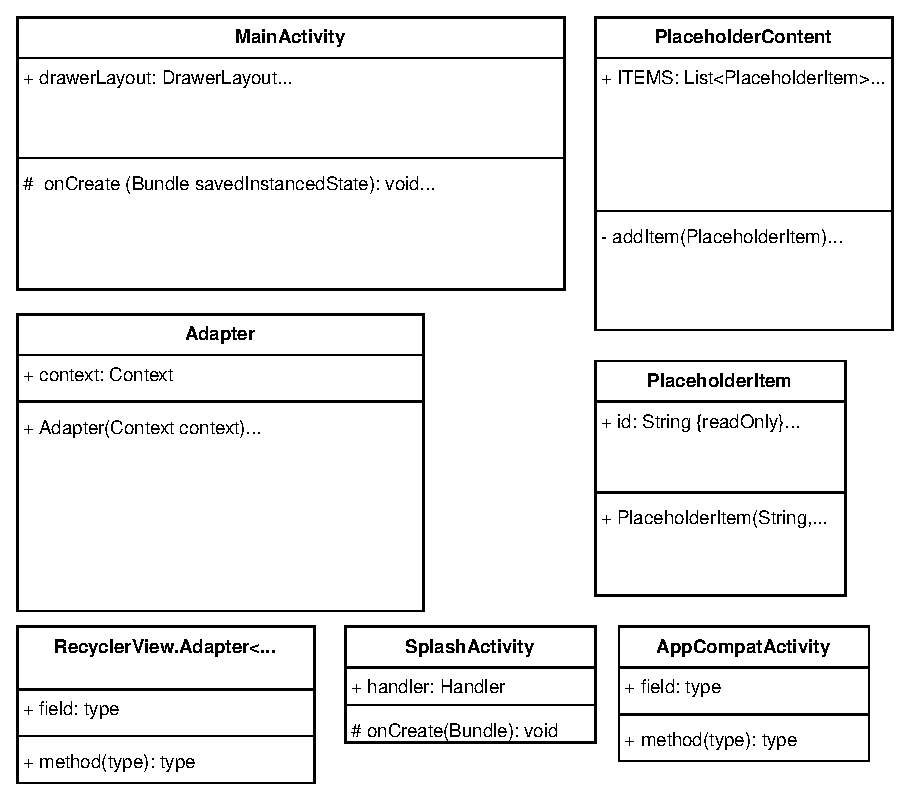
\includegraphics[width=\textwidth]{Diagrams/Class Diagrams/Class Diagram-Other Classes}
        \caption{Class Diagram: Other}
        \label{fig:figure4}
    \end{figure}

    Contains all classes \textbf{not} already included in the other diagrams above.
    Relationships included only as part of \textit{Class Diagram: Medication}.
    \pagebreak


    \section{State-machine diagram}\label{sec:state-machine-diagram}

    \begin{figure}[H]
        \centering
        \includegraphics[width=\textwidth]{Diagrams/State Diagram/State Diagram}
        \caption{State Diagram: Whole System}
        \label{fig:figure5}
    \end{figure}

    Contains the state diagram of the whole system.
    Each specific screen in the UI interface being its own composite state.
    Each composite state has substrates, however they all follow the user interaction $\rightarrow$ system reaction pattern.

    %for the whole system if possible
    \pagebreak


    \section{Entity Relationship Diagram (Data modelling)}\label{sec:er--diagram-(data-modelling)}

    \begin{figure}[H]
        \centering
        \includegraphics[width=\textwidth]{Diagrams/Entity Relationship Diagram}
        \caption{Entity Relationship Diagram}
        \label{fig:figure6}
    \end{figure}

    The entity relationship diagram (Data modelling) for the system.

    \pagebreak


    \section{GitHub Link}\label{sec:github-link}

    \textbf{You MUST ask Yonatan Alexander for access, as this repository is set to private.}\\

    \href{https://github.com/Jon-AL/4471---Therapy-Support-App}{Group Therapy-Support-App}


    \section{Conclusion}\label{sec:conclusion}

    In many ways, the project did not go according to plan.
    We made a number of mistakes, but we believe the biggest was not making the project in Kotlin.
    Making the project in Kotlin would have allowed us to make the app's UI programmatically, which would have been a huge improvement.
    Additionally, this project turned out to be far larger in scope than we anticipated, simply because we were learning as we went.

    In summary, many mistakes were made, but making such mistakes in a project where the intention is learning is exactly the right time to make them - and therefore we believe that those mistakes were (overall, at least) a positive.

    \pagebreak


    \section{References}\label{sec:reference}

    \begin{enumerate}
        [label=\[\arabic*\]]
        \item \textbf{Smartpatient} (nd) \textsl{MyTherapy} (app): ``Your personal pill reminder and medication tracker app'', \href{www.mytherapyapp.com}{MyTherapy}

        \item \textbf{Bipolar UK} (nd) \textsl{Bipolar UK’s Mood Tracker} (app): ``Our new Mood Tracker app can make it much easier to record your daily mood, medications, emotions and how much sleep you’ve had'', \href{https://www.bipolaruk.org/blog/track-your-mood-app}{Bipolar UK}

    \end{enumerate}


    \pagebreak


    \appendix

    \appendixpage


    \section{Project WBS and Gantt Chart}\label{sec:project-wbs}

    \subsection{Project WBS}\label{subsec:project-wbs}

    Spread over a number of pages due to Project Libre's many limitations

    \begin{figure}[H]
        \centering
        \includegraphics[width=\textwidth]{ProjectLibre/WBS as PNG/Pages from My Mental Health App WBS-5_Page_1}
        \caption{WBS Part 1 out of 5}
        \label{fig:figure7}
    \end{figure}

    \begin{figure}[H]
        \centering
        \includegraphics[width=\textwidth]{ProjectLibre/WBS as PNG/Pages from My Mental Health App WBS-5_Page_2}
        \caption{WBS Part 2 out of 5}
        \label{fig:figure8}
    \end{figure}

    \begin{figure}[H]
        \centering
        \includegraphics[width=\textwidth]{ProjectLibre/WBS as PNG/Pages from My Mental Health App WBS-5_Page_3}
        \caption{WBS Part 3 out of 5}
        \label{fig:figure9}
    \end{figure}

    \begin{figure}[H]
        \centering
        \includegraphics[width=\textwidth]{ProjectLibre/WBS as PNG/Pages from My Mental Health App WBS-5_Page_4}
        \caption{WBS Part 4 out of 5}
        \label{fig:figure10}
    \end{figure}

    \begin{figure}[H]
        \centering
        \includegraphics[width=\textwidth]{ProjectLibre/WBS as PNG/Pages from My Mental Health App WBS-5_Page_5}
        \caption{WBS Part 5 out of 5}
        \label{fig:figure11}
    \end{figure}
%    \includegraphics[angle=90,origin=c]{file}
%    \includepdf[pages=-]{ProjectLibre/My Mental Health App WBS.pdf}

    \subsection{Project Gantt Chart}\label{subsec:project-gantt-chart}

    \begin{figure}[H]
        \centering
        \includegraphics[angle=90,origin=c,height=0.7\textheight]{ProjectLibre/My Mental Health App Gantt}
        \caption{Gantt Chart}
        \label{fig:figure12}
    \end{figure}
%    \includepdf[pages=-]{ProjectLibre/My Mental Health App.pdf}

    \pagebreak


    \section{Task Assignment Matrix}\label{sec:task-assignment-matrix}
    \begin{table}[H]
        \centering
        \begin{tabular}{lll}
            \toprule
            \textbf{Task}                      & \textbf{Task Owner} & \textbf{Support} \\
            \midrule
            Basic UI User Interfaces           & Yasin               & Yonatan, Michael \\
            User Stories for Project UI        & Yasin               & Yonatan, Michael \\
            Advanced UI User Interfaces        & Michael             & Yonatan          \\
            Front end (UI) completion          & Michael             & Yonatan          \\
            WBS                                & Yonatan, Michael    &                  \\
            Gantt Chart                        & Michael, Yonatan    &                  \\
            Task Assignment Matrix             & Yonatan, Michael    &                  \\
            Testing Matrix                     & Michael             & Yonatan          \\
            Skeleton Code                      & Yonatan             & Michael          \\
            Database Integration with Backend  & Yonatan, Michael    &                  \\
            Database Execution                 & Michael             & Yonatan          \\
            Front end Integration with Backend & Michael             & Yonatan          \\
            Use Case Diagrams                  & Yonatan, Michael    &                  \\
            Use Case Descriptions              & Michael             & Yonatan          \\
            Sequence Diagrams                  & Yonatan, Michael    &                  \\
            Class Diagram                      & Yonatan, Michael    &                  \\
            Data Entity Relationship Diagram   & Yonatan, Michael    &                  \\
            State Diagrams                     & Michael             & Yonatan          \\
            Video                              & Yonatan             & Michael          \\
            Slideshow                          & Michael, Yonatan    &                  \\
            Report Editing                     & Yonatan             & Michael          \\
            \bottomrule
        \end{tabular}
        \caption{Task Assignment Matrix}\label{tab:table}
    \end{table}

    \textsl{This table reflects what happened in practice, not what the plan was initially.}

    \begin{figure}
        \label{fig:Gant Chart} %GANT CHART
    \end{figure}
    \pagebreak


    \section{The History of Commits}\label{sec:the-history-of-commits}

    \textsl{Does not contain the very latest commits, only the almost very latest commits.}

    \begin{center}
        \begin{longtable}{|p{2cm}|l|p{2cm}|p{10.5cm}|}
            \caption{\textbf{Almost Complete Commit History}} \label{tab:long} \\

            \hline \multicolumn{1}{|c|}{\textbf{Date}} & \multicolumn{1}{c|}{\textbf{Time}} & \multicolumn{1}{c|}{\textbf{Committer}}& \multicolumn{1}{c|}{\textbf{Note}} \\ \hline
            \endfirsthead

            \multicolumn{4}{c}%
            {{\bfseries \tablename\ \thetable{} -- continued from previous page}} \\
            \hline \multicolumn{1}{|c|}{\textbf{Date}} & \multicolumn{1}{c|}{\textbf{Time}} & \multicolumn{1}{c|}{\textbf{Committer}}& \multicolumn{1}{c|}{\textbf{Note}} \\ \hline
            \endhead

            \hline \multicolumn{4}{|r|}{{Continued on next page}} \\ \hline
            \endfoot

            \hline \hline
            \endlastfoot
            03-12-2022                                 & 03:13                              & Jon-AL                                  & This time, really the Last Update :)                                                                                                                                                                                                                                                                         \\ \hline
            03-12-2022                                 & 02:32                              & Jon-AL                                  & Last Update :)                                                                                                                                                                                                                                                                                               \\ \hline
            03-12-2022                                 & 02:14                              & Jon-AL                                  & tiny updates                                                                                                                                                                                                                                                                                                 \\ \hline
            03-12-2022                                 & 02:12                              & Jon-AL                                  & deleted uneeded files (WBS png and svg)                                                                                                                                                                                                                                                                      \\ \hline
            03-12-2022                                 & 02:11                              & Jon-AL                                  & main.tax updated to contain the Gantt chart and the WBS in a more accessible manner. File organization (preparing for submission), README.md update                                                                                                                                                          \\ \hline
            03-12-2022                                 & 01:02                              & Jon-AL                                  & README.md update                                                                                                                                                                                                                                                                                             \\ \hline
            03-12-2022                                 & 01:01                              & Jon-AL                                  & README.md update                                                                                                                                                                                                                                                                                             \\ \hline
            03-12-2022                                 & 01:00                              & Jon-AL                                  & README.md update                                                                                                                                                                                                                                                                                             \\ \hline
            03-12-2022                                 & 00:51                              & Jon-AL                                  & README.txt->README.md                                                                                                                                                                                                                                                                                        \\ \hline
            03-12-2022                                 & 00:49                              & Jon-AL                                  & Organizing the files                                                                                                                                                                                                                                                                                         \\ \hline
            03-12-2022                                 & 00:46                              & Jon-AL                                  & Starting organizing the files                                                                                                                                                                                                                                                                                \\ \hline
            03-12-2022                                 & 00:44                              & Jon-AL                                  & Revert ``Starting organizing the files''                                                                                                                                                                                                                                                                     \\ \hline
            03-12-2022                                 & 00:44                              & Jon-AL                                  & Starting organizing the files                                                                                                                                                                                                                                                                                \\ \hline
            03-12-2022                                 & 00:40                              & Jon-AL                                  & Starting organizing the files                                                                                                                                                                                                                                                                                \\ \hline
            03-12-2022                                 & 00:34                              & Jon-AL                                  & Re-committed LaTeX                                                                                                                                                                                                                                                                                           \\ \hline
            03-12-2022                                 & 00:33                              & Jon-AL                                  & Merge branch `main' into michael\_workingbranch                                                                                                                                                                                                                                                              \\ \hline
            02-12-2022                                 & 23:16                              & Jon-AL                                  & Updated LaTeX in branch                                                                                                                                                                                                                                                                                      \\ \hline
            02-12-2022                                 & 22:57                              & Michael                                 & Updated comments.                                                                                                                                                                                                                                                                                            \\ \hline
            02-12-2022                                 & 22:09                              & Michael                                 & Merge branch `main' of https://github.com/Jon-AL/4471---Therapy-Support-App                                                                                                                                                                                                                                  \\ \hline
            02-12-2022                                 & 22:06                              & Michael                                 & pushed testcases                                                                                                                                                                                                                                                                                             \\ \hline
            02-12-2022                                 & 21:55                              & Michael                                 & Update README.txt                                                                                                                                                                                                                                                                                            \\ \hline
            02-12-2022                                 & 21:49                              & Michael                                 & Update README.txt                                                                                                                                                                                                                                                                                            \\ \hline
            02-12-2022                                 & 21:44                              & Michael                                 & Update README.txt                                                                                                                                                                                                                                                                                            \\ \hline
            02-12-2022                                 & 20:59                              & Michael                                 & Changed the text entered times.                                                                                                                                                                                                                                                                              \\ \hline
            02-12-2022                                 & 20:49                              & Michael                                 & Changed the text entered times.                                                                                                                                                                                                                                                                              \\ \hline
            02-12-2022                                 & 19:57                              & Michael                                 & Merge remote-tracking branch `origin/main'                                                                                                                                                                                                                                                                   \\ \hline
            02-12-2022                                 & 19:57                              & Michael                                 & Massive comment push.                                                                                                                                                                                                                                                                                        \\ \hline
            02-12-2022                                 & 19:43                              & Jon-AL                                  & Merge remote-tracking branch `origin/michael\_workingbranch' into michael\_workingbranch                                                                                                                                                                                                                     \\ \hline
            02-12-2022                                 & 19:43                              & Jon-AL                                  & Project Report Updated (Nearly done), added class diagrams                                                                                                                                                                                                                                                   \\ \hline
            02-12-2022                                 & 18:51                              & Michael                                 & Added a build readme file.                                                                                                                                                                                                                                                                                   \\ \hline
            02-12-2022                                 & 18:15                              & Michael                                 & Had to change the gradle file.                                                                                                                                                                                                                                                                               \\ \hline
            02-12-2022                                 & 15:38                              & Michael                                 & Bugs were patched after the introduction of test case file.                                                                                                                                                                                                                                                  \\ \hline
            02-12-2022                                 & 11:11                              & Michael                                 & Bug fixes have been fixed, and app modifications have been changed. The home screen is now the add screen. Defensive statements have been added to reject non-valid empty fields.                                                                                                                            \\ \hline
            02-12-2022                                 & 00:21                              & Michael                                 & Merge branch `michael\_workingbranch'                                                                                                                                                                                                                                                                        \\ \hline
            02-12-2022                                 & 00:20                              & Michael                                 & fragment bug fix.                                                                                                                                                                                                                                                                                            \\ \hline
            01-12-2022                                 & 23:32                              & Jon-AL                                  & Merge remote-tracking branch `origin/michael\_workingbranch' into michael\_workingbranch                                                                                                                                                                                                                     \\ \hline
            01-12-2022                                 & 23:32                              & Jon-AL                                  & Project Report Updated, added class diagrams                                                                                                                                                                                                                                                                 \\ \hline
            01-12-2022                                 & 23:24                              & Michael                                 & Merge branch `michael\_workingbranch'                                                                                                                                                                                                                                                                        \\ \hline
            01-12-2022                                 & 23:15                              & Michael                                 & rcmenu was forgotten. it needs to be placed inside there.                                                                                                                                                                                                                                                    \\ \hline
            01-12-2022                                 & 23:14                              & Michael                                 & Cleaned up code and commented some left behind functions. More comments can possibly happen tomorrow or tonight.                                                                                                                                                                                             \\ \hline
            01-12-2022                                 & 20:48                              & Michael                                 & Merge branch `michael\_workingbranch' of https://github.com/Jon-AL/4471---Therapy-Support-App into michael\_workingbranch                                                                                                                                                                                    \\ \hline
            01-12-2022                                 & 20:48                              & Michael                                 & Revised Detailed Class Diagram                                                                                                                                                                                                                                                                               \\ \hline
            01-12-2022                                 & 20:18                              & Jon-AL                                  & Project Report Updated                                                                                                                                                                                                                                                                                       \\ \hline
            01-12-2022                                 & 20:01                              & Jon-AL                                  & Project Report Updated                                                                                                                                                                                                                                                                                       \\ \hline
            01-12-2022                                 & 19:08                              & Michael                                 & Updated comments with partially finished UML diagram.                                                                                                                                                                                                                                                        \\ \hline
            01-12-2022                                 & 18:06                              & Michael                                 & storing current changes so nothing is lost.                                                                                                                                                                                                                                                                  \\ \hline
            01-12-2022                                 & 15:01                              & Michael                                 & Updated use case and sequence diagrams.                                                                                                                                                                                                                                                                      \\ \hline
            01-12-2022                                 & 11:16                              & Michael                                 & Updated comments for mooddb helper and fragment had its refresh button resized to make the UI cleaner.                                                                                                                                                                                                       \\ \hline
            01-12-2022                                 & 11:07                              & Michael                                 & Updated all the medication views to make it look much nicer.                                                                                                                                                                                                                                                 \\ \hline
            01-12-2022                                 & 09:30                              & Michael                                 & Updated medication view. delete and update methods are buggy atm.                                                                                                                                                                                                                                            \\ \hline
            01-12-2022                                 & 01:44                              & Michael                                 & Fixed medicaTION VIEW                                                                                                                                                                                                                                                                                        \\ \hline
            30-11-2022                                 & 22:07                              & Michael                                 & Cleaned up portions of code.                                                                                                                                                                                                                                                                                 \\ \hline
            30-11-2022                                 & 19:34                              & Michael                                 & A lot of code except reports has been commented.                                                                                                                                                                                                                                                             \\ \hline
            30-11-2022                                 & 18:16                              & Michael                                 & UI rebuild.                                                                                                                                                                                                                                                                                                  \\ \hline
            30-11-2022                                 & 17:31                              & Michael                                 & Suggestions of removing bar and adding comments added in this version.                                                                                                                                                                                                                                       \\ \hline
            29-11-2022                                 & 01:09                              & Michael                                 & A simple bar graph has been pushed into the mood report code. ty yonatan                                                                                                                                                                                                                                     \\ \hline
            28-11-2022                                 & 23:07                              & Jon-AL                                  & added gradle support for a couple of external libraries                                                                                                                                                                                                                                                      \\ \hline
            28-11-2022                                 & 22:45                              & Jon-AL                                  & small modifications to mood addition frag                                                                                                                                                                                                                                                                    \\ \hline
            28-11-2022                                 & 22:36                              & Michael                                 & Mood had its update method split into the addition component. The read and delete methods are two different components.                                                                                                                                                                                      \\ \hline
            28-11-2022                                 & 22:28                              & Michael                                 & Mood had its update method split into the addition component. The read and delete methods are two different components.                                                                                                                                                                                      \\ \hline
            28-11-2022                                 & 21:57                              & Michael                                 & med list updated.                                                                                                                                                                                                                                                                                            \\ \hline
            28-11-2022                                 & 21:53                              & Michael                                 & med list updated.                                                                                                                                                                                                                                                                                            \\ \hline
            28-11-2022                                 & 21:51                              & Michael                                 & med list updated.                                                                                                                                                                                                                                                                                            \\ \hline
            28-11-2022                                 & 21:19                              & Michael                                 & Separated the add button.                                                                                                                                                                                                                                                                                    \\ \hline
            28-11-2022                                 & 19:53                              & Michael                                 & Updated data to revert crash. Pushed to save current work.                                                                                                                                                                                                                                                   \\ \hline
            28-11-2022                                 & 17:31                              & Jon-AL                                  & + to mood                                                                                                                                                                                                                                                                                                    \\ \hline
            27-11-2022                                 & 21:32                              & Michael                                 & Seek bar color is dynamically changing as the seek bar motion is changing.                                                                                                                                                                                                                                   \\ \hline
            27-11-2022                                 & 10:10                              & Michael                                 & Seek bar is now working with the short description, rating, and long description. This progress is being committed to avoid the app crashing during the report development.                                                                                                                                  \\ \hline
            27-11-2022                                 & 06:48                              & Michael                                 & Merge branch `michael\_workingbranch'                                                                                                                                                                                                                                                                        \\ \hline
            27-11-2022                                 & 06:46                              & Michael                                 & Seek bar is now working with the short description, rating, and long description. This progress is being committed to avoid the app crashing during the report development.                                                                                                                                  \\ \hline
            27-11-2022                                 & 06:25                              & Michael                                 & Temporary fix for mood.                                                                                                                                                                                                                                                                                      \\ \hline
            26-11-2022                                 & 23:58                              & Michael                                 & Mood has been significantly updated. The slider works with the new addition method. Read and delete are now functional. Delete has an updated primary key. Update is not working at this point in time.                                                                                                      \\ \hline
            26-11-2022                                 & 21:43                              & Michael                                 & Updated the current plus to have a working a visual sliding bar as requested. Code and descriptions was pulled from Yonatan`s code.                                                                                                                                                                          \\ \hline
            26-11-2022                                 & 20:38                              & Michael                                 & Merge branch `michael\_workingbranch'                                                                                                                                                                                                                                                                        \\ \hline
            26-11-2022                                 & 20:29                              & Michael                                 & This is protect what work we have from changes.                                                                                                                                                                                                                                                              \\ \hline
            26-11-2022                                 & 12:26                              & Jonathan                                & added seek bar, minor updates                                                                                                                                                                                                                                                                                \\ \hline
            25-11-2022                                 & 10:17                              & Jon-AL                                  & PPTX                                                                                                                                                                                                                                                                                                         \\ \hline
            24-11-2022                                 & 22:06                              & Jon-AL                                  & Corrected a color                                                                                                                                                                                                                                                                                            \\ \hline
            24-11-2022                                 & 22:03                              & Jon-AL                                  & Corrected a color                                                                                                                                                                                                                                                                                            \\ \hline
            24-11-2022                                 & 20:28                              & Jon-AL                                  & Merge branch `jonathan'                                                                                                                                                                                                                                                                                      \\ \hline
            24-11-2022                                 & 16:48                              & Jon-AL                                  & New Logo New color scheme                                                                                                                                                                                                                                                                                    \\ \hline
            24-11-2022                                 & 12:20                              & Jon-AL                                  & Switching branch, requires commit first.                                                                                                                                                                                                                                                                     \\ \hline
            23-11-2022                                 & 17:59                              & Michael                                 & Updated Use Case diagrams                                                                                                                                                                                                                                                                                    \\ \hline
            21-11-2022                                 & 19:26                              & Michael                                 & Medication code has been created. Update, add and delete seem to work but the view does not fit.                                                                                                                                                                                                             \\ \hline
            21-11-2022                                 & 19:12                              & Michael                                 & Medication code has been created. Update, add and delete seem to work but the view does not fit.                                                                                                                                                                                                             \\ \hline
            21-11-2022                                 & 16:57                              & Michael                                 & Medication Modal and Medication DB code modified.                                                                                                                                                                                                                                                            \\ \hline
            21-11-2022                                 & 15:41                              & Michael                                 & Symptom base feature has been established, created, and implemented db as the prof suggested.                                                                                                                                                                                                                \\ \hline
            21-11-2022                                 & 14:20                              & Michael                                 & Fragments medication and symptom have been started. No connection as of yet.                                                                                                                                                                                                                                 \\ \hline
            21-11-2022                                 & 14:12                              & Michael                                 & Modals have been created for base features Medication and Symptom.                                                                                                                                                                                                                                           \\ \hline
            21-11-2022                                 & 13:24                              & Michael                                 & All initial features are done for mood.                                                                                                                                                                                                                                                                      \\ \hline
            18-11-2022                                 & 09:24                              & Michael                                 & VCiew and delete method being worked on.                                                                                                                                                                                                                                                                     \\ \hline
            18-11-2022                                 & 08:31                              & Michael                                 & View method being worked on.                                                                                                                                                                                                                                                                                 \\ \hline
            18-11-2022                                 & 00:37                              & Michael                                 & Adding data is possible now. Reading the data is crashing. Delete method is not up yet.                                                                                                                                                                                                                      \\ \hline
            16-11-2022                                 & 21:45                              & Michael                                 & App is no longer crashing. Fragment layout is displaying but stuck on how to change the activity into a fragment.                                                                                                                                                                                            \\ \hline
            14-11-2022                                 & 19:31                              & Michael                                 & Something keeps shutting the app down when the database is installed. Do not run at this time.                                                                                                                                                                                                               \\ \hline
            14-11-2022                                 & 14:21                              & Michael                                 & Merge branch `main' into michael\_workingbranch                                                                                                                                                                                                                                                              \\ \hline
            12-11-2022                                 & 20:41                              & Mohammad Yasin Aziz                     & First Commit. Commit No 1. Created skeleton UI so that the backend dev can start working. 12 Nov 2022                                                                                                                                                                                                        \\ \hline
            07-11-2022                                 & 20:50                              & Michael                                 & Database has an updated delete method for a single record, and a method for dropping the table. Experimental.                                                                                                                                                                                                \\ \hline
            07-11-2022                                 & 11:20                              & Jon-AL                                  & Added the `loading' screen                                                                                                                                                                                                                                                                                   \\ \hline
            07-11-2022                                 & 09:33                              & Jon-AL                                  & Large commit; changed organization of files slightly (androidTest->main). Added new activity for main menu.                                                                                                                                                                                                  \\ \hline
            06-11-2022                                 & 22:41                              & Mohammad Yasin Aziz                     & Add files via upload                                                                                                                                                                                                                                                                                         \\ \hline
            06-11-2022                                 & 20:43                              & Michael                                 & Updated use case and entity relationship diagram.                                                                                                                                                                                                                                                            \\ \hline
            06-11-2022                                 & 20:42                              & Michael                                 & Previous upload was not correctly updated. My bad.                                                                                                                                                                                                                                                           \\ \hline
            06-11-2022                                 & 20:41                              & Michael                                 & Updated use case diagram. An addition of the entity relationship diagram (rough copy).                                                                                                                                                                                                                       \\ \hline
            06-11-2022                                 & 16:37                              & Michael                                 & Important line for writing to a database had to be written in AndroidManifest.xml                                                                                                                                                                                                                            \\ \hline
            06-11-2022                                 & 16:36                              & Michael                                 & Updated a sample interface on how the user would interact with the app.                                                                                                                                                                                                                                      \\ \hline
            06-11-2022                                 & 16:01                              & Michael                                 & Use Case diagram change                                                                                                                                                                                                                                                                                      \\ \hline
            06-11-2022                                 & 15:59                              & Michael                                 & Cleaned up mood db and symptom db to remove db table ambiguity. An additional variable was created to make symptom db more representative of current database labelled inside diagrams.                                                                                                                      \\ \hline
            05-11-2022                                 & 18:43                              & Michael                                 & Mood db for now. Functionality will come later.                                                                                                                                                                                                                                                              \\ \hline
            05-11-2022                                 & 18:34                              & Michael                                 & MedicationDBHelper.java has removed a useless library and variable comment.                                                                                                                                                                                                                                  \\ \hline
            05-11-2022                                 & 16:19                              & Michael                                 & Further comments at the start.                                                                                                                                                                                                                                                                               \\ \hline
            05-11-2022                                 & 16:18                              & Michael                                 & Initial creation of MedicationDBHelper.java. This class will support medication for now. Base feature of creating and adding the database has been established.                                                                                                                                              \\ \hline
            04-11-2022                                 & 14:26                              & Jon-AL                                  & Medication - draft class to be used by graphical interface to display medications.                                                                                                                                                                                                                           \\ \hline
            04-11-2022                                 & 14:26                              & Jon-AL                                  & NumericMoodCheckIn - class to be used by graphical interface. Does it's own conversion from number to descriptors (short, long). To be made into a UI component for self reporting. Text take from the app ``Bi-Polar UK'', may need to be changed/updated according to the current psychological standards. \\ \hline
            02-11-2022                                 & 17:57                              & Jon-AL                                  & re-synced patterns                                                                                                                                                                                                                                                                                           \\ \hline
            02-11-2022                                 & 17:55                              & Jon-AL                                  & Updated visuals in title                                                                                                                                                                                                                                                                                     \\ \hline
            02-11-2022                                 & 10:18                              & Jon-AL                                  & Updated visuals in title                                                                                                                                                                                                                                                                                     \\ \hline
            02-11-2022                                 & 09:31                              & Jon-AL                                  & Merge remote-tracking branch `origin/main' into jonathan                                                                                                                                                                                                                                                     \\ \hline
            02-11-2022                                 & 09:30                              & Jon-AL                                  & Updated visuals in title                                                                                                                                                                                                                                                                                     \\ \hline
            01-11-2022                                 & 23:05                              & Michael                                 & Merge pull request \#2 from Jon-AL/michael\_workingbranch                                                                                                                                                                                                                                                    \\ \hline
            01-11-2022                                 & 23:04                              & Michael                                 & Merge pull request \#1 from Jon-AL/jonathan                                                                                                                                                                                                                                                                  \\ \hline
            01-11-2022                                 & 17:01                              & Jon-AL                                  & Updated visuals in title                                                                                                                                                                                                                                                                                     \\ \hline
            01-11-2022                                 & 16:55                              & Jon-AL                                  & Updated visuals in title                                                                                                                                                                                                                                                                                     \\ \hline
            01-11-2022                                 & 12:31                              & Jon-AL                                  & design pattern templates for future reference (src: refactoring\_guru)                                                                                                                                                                                                                                       \\ \hline
            01-11-2022                                 & 11:50                              & Jon-AL                                  & App bones commit                                                                                                                                                                                                                                                                                             \\ \hline
            01-11-2022                                 & 11:49                              & Jon-AL                                  & Main file                                                                                                                                                                                                                                                                                                    \\ \hline
            01-11-2022                                 & 11:27                              & Jon-AL                                  & Main file                                                                                                                                                                                                                                                                                                    \\ \hline
            01-11-2022                                 & 11:23                              & Jon-AL                                  & Main file                                                                                                                                                                                                                                                                                                    \\ \hline
            01-11-2022                                 & 10:59                              & Jon-AL                                  & Main file                                                                                                                                                                                                                                                                                                    \\ \hline
            07-10-2022                                 & 13:05                              & Jonathan                                & Updated sections, TOC, started on Bib                                                                                                                                                                                                                                                                        \\ \hline
            07-10-2022                                 & 13:04                              & Jonathan                                & Updated sections, TOC, started on Bib                                                                                                                                                                                                                                                                        \\ \hline
            07-10-2022                                 & 10:33                              & Jonathan                                & Main file                                                                                                                                                                                                                                                                                                    \\ \hline
            07-10-2022                                 & 10:32                              & Jonathan                                & Merge branch `michael\_workingbranch' of https://github.com/Jon-AL/4471---Therapy-Support-App into jonathan                                                                                                                                                                                                  \\ \hline
            07-10-2022                                 & 10:28                              & Jonathan                                & Main file                                                                                                                                                                                                                                                                                                    \\ \hline
            05-10-2022                                 & 17:37                              & Michael                                 & Add files via upload                                                                                                                                                                                                                                                                                         \\ \hline
            05-10-2022                                 & 17:34                              & Michael                                 & Add files via upload                                                                                                                                                                                                                                                                                         \\ \hline
            04-10-2022                                 & 13:38                              & Jon-AL                                  & Main file                                                                                                                                                                                                                                                                                                    \\ \hline
            04-10-2022                                 & 13:26                              & Jon-AL                                  & Merge remote-tracking branch `origin/main'                                                                                                                                                                                                                                                                   \\ \hline
            04-10-2022                                 & 13:26                              & Jon-AL                                  & Deleted duplicate file                                                                                                                                                                                                                                                                                       \\ \hline
            04-10-2022                                 & 13:25                              & Jon-AL                                  & Deleted duplicate file                                                                                                                                                                                                                                                                                       \\ \hline
            04-10-2022                                 & 13:20                              & Jon-AL                                  & Main file                                                                                                                                                                                                                                                                                                    \\ \hline
            04-10-2022                                 & 13:19                              & Jon-AL                                  & Main file                                                                                                                                                                                                                                                                                                    \\ \hline
            04-10-2022                                 & 13:17                              & Jon-AL                                  & Add files via upload                                                                                                                                                                                                                                                                                         \\


        \end{longtable}
    \end{center}

    \pagebreak


%    \section{Wants}
%
%    The following were not added to the system.
%
%    \begin{enumerate}
%        \item docker
%        \item gant chart
%        \item Reminder system
%        \item Privacy
%        \item Minutes
%        \item Encryption for data (including for local storage)
%        \begin{itemize}
%            \item Was implemented as part of Android since Android 11.
%        \end{itemize}
%        \item Login system
%        \item Therapist interface
%    \end{enumerate}
%    \pagebreak


    \section{Minutes}

    \subsection{26-Sep-’22}\label{subsec:26-sep-22}

    \textbf{Present:}
    \begin{itemize}
        \item Yonatan
        \item Michael
    \end{itemize}

    \textbf{Not Present:}

    \begin{itemize}
        \item Yasin
    \end{itemize}

    \textbf{Discussed:}

    \begin{itemize}
        \item  Development proposal and development details.
        \item  The project will be a therapy application that helps users gather, store and present their information to be used by patients.
        \item Suggested so far:
        \begin{itemize}
            \item Incremental development.
            \item Smartphone app.
            \item Web app.
        \end{itemize}
        \item  Suggested Programming languages:
        \begin{itemize}
            \item Dart.
            \item Python.
            \item Javascript.
            \item C++.
            \item Java.
        \end{itemize}
        \item Stakeholders:
        \begin{itemize}
            \item Clients.
            \item Therapists and other mental health professionals.
        \end{itemize}
        \item Features:
        \begin{itemize}
            \item Mood self-reported values.
            \item Medication tracking.
        \end{itemize}

    \end{itemize}

    \subsection{30-Sep-’22}\label{subsec:30-sep-22}

    \textbf{Present:}
    \begin{itemize}
        \item Yonatan
        \item Michael
    \end{itemize}

    \textbf{Not Present:}

    \begin{itemize}
        \item Yasin
    \end{itemize}

    \textbf{Discussed:}

    \begin{itemize}
        \item Project proposal was accepted.
        \item Instructor mentioned a number of points during lecture in the context of our project:
        \begin{itemize}
            \item Patient data requirements with respect to privacy.
            \item Identifying the stakeholders with who should be able to access data.
            \item We need to identify the use cases carefully of what we are able to do.
            \item We have to be able to clearly define the project objective and description.
        \end{itemize}
        \item An aggressive timeline has been suggested to keep with coursework.
        This timeline is subject to change due to other courses requiring our attention.
        \item Github was setup by Yonatan.
        \item Report is in progress.
    \end{itemize}

    \subsection{04-Oct-’22 and 05-Oct-’22}

    \textbf{Discussed:}

    A timeline has been suggested to be finishing up to the user acceptance criteria.
    QT has been suggested as a platform to build an Android app.

    The report has been started in LaTex by Yonatan.
    Proposed statements will be made by the group once we reviewed the work.

    \subsection{14-Oct-’22}

    \textbf{Present:}
    \begin{itemize}
        \item Yonatan
        \item Michael
        \item Yasin
    \end{itemize}

    \textbf{Discussed:}

    Debate about the code is that we have no firm agreements on project libraries and frameworks.
    Suggestions include: salesforce as the backend.
    Flutter or ReactNative has also been suggested.
    Qt.

    \subsection{21-Oct-’22 to 28-Oct-’22}\label{subsec:21-oct-22-to-28-oct-22}


    A lot of project will be developed on the reading week.
    Professor wants us to use Docker, and create a Gantt chart.
    He explicitly states that he wants us to assign backup roles to our task assignment matrix.

    \subsection{01-Nov-’22}\label{subsec:01-nov-22}

    \textbf{Present:}
    \begin{itemize}
        \item Yonatan
        \item Michael
    \end{itemize}

    \textbf{Not Present:}

    \begin{itemize}
        \item Yasin
    \end{itemize}

    \textbf{Discussed:}

    \item    Planned architecture:
    \begin{itemize}
        \begin{itemize}
            \item repository style for the databases.
            \item Event-driven for reminders.
            \item Component-based.
        \end{itemize}
        \item Today's objective:
        \begin{itemize}
            \item Architecture and design patterns were discussed.
            \item Get the backend done behind the scenes.
            \item Another meeting: 9:30 am to 11:30 am tomorrow (November 2nd, 2022), want to start writing code.
        \end{itemize}
    \end{itemize}

    \subsection{02-Nov-’22}\label{subsec:02-nov-222}

    \textbf{Present:}
    \begin{itemize}
        \item Yonatan
        \item Michael
    \end{itemize}


    \textbf{Not Present:}

    \begin{itemize}
        \item Yasin
    \end{itemize}

    \textbf{Discussed:}
    \begin{itemize}
        \item We are switching the development process from incremental to a hybrid agile-iterative method.
        \item Scope and requirements changed significantly throughout the process.
        \item We are also incorporating agile methods to respond to changes over time.
        \item Kanban board has been created inside GitHub repository.
        \item User stories will be created for UI to make the interface clearer to write components and understand the problems.
        \item Drafts have been started but significant changes need to be created.
        \item An Android application will be created.
        \item The data will be stored locally with some encryption to get us started.
        \item Yonatan wants to push simple skeleton code, will require approval from Michael and Yasin.
        \item We want to finish baseline features executed and finished by November 6th.
        \item The list of things we want executed:
        \begin{itemize}
            \item A basic UI - covered by Yasin (done).
            \item Basic backend - covered by Yonatan
            \item Database integration - covered by Michael
        \end{itemize}
        \item We will need significant research need before implementations.
        \item No meeting will be scheduled for tomorrow.
        \item A few mini-meetings between Friday to Sunday.
    \end{itemize}

    \subsection{02-Nov-’22}\label{subsec:02-nov-22}

    \textbf{Present:}
    \begin{itemize}
        \item Yonatan
        \item Michael
    \end{itemize}

    \textbf{Not Present:}

    \begin{itemize}
        \item Yasin
    \end{itemize}

    \textbf{Discussed:}
    \begin{itemize}
        \item Backend talk
        \item Significant modifications need to be executed for medication.
        \item We will have to split this into 3 main Tables:
        \begin{enumerate}
            \item Medication info
            \item Medication inventory history
            \item Medication intake history
        \end{enumerate}
        \item Mood will be generated next.
        \item Symptoms will be generated last.
        \item Backend sample is expected to be done by Sunday late afternoon.
        \item Yasin will present a frontend demo on November 6th.
    \end{itemize}

    \subsection{14-Nov-’22}\label{subsec:14-nov-22}

    \textbf{Present:}
    \begin{itemize}
        \item Yonatan
        \item Michael
        \item Yasin
    \end{itemize}

    \textbf{Discussed:}
    \begin{itemize}
        \item  Front end and back end are being implemented.
        We are integrating today.
        \item  Our approach has changed.
        We have recognized that the Model-View-ViewModel (MVVM) pattern was the best representation.
        \item Things to do:
        \begin{itemize}
            \item Integrate front-end and back-end.
            \item Revise databases.
            \item Check on scope and extra features.
            \item Testing and presentation notes to build.
        \end{itemize}
    \end{itemize}

    \subsection{24-Nov-’22}\label{subsec:24-nov-22}
    \textbf{Present:}
    \begin{itemize}
        \item Yonatan
        \item Michael
    \end{itemize}

    \textbf{Not Present:}

    \begin{itemize}
        \item Yasin
    \end{itemize}

    \textbf{Discussed:}

    \begin{itemize}
        \item
        \item Presentation is being worked on.
        \item Yonatan changed color scheme and logo.
        \item Things to do:
        \begin{enumerate}
            \item  He wants a better option for moods.
            A better option would be spinner or radio button.
            A perfect solution would be adding a slider [Seek bar].
            \item  We need to focus more on accessibility.
            \item  Add statistics.
        \end{enumerate}
    \end{itemize}

    \subsection{27-Nov-’22}\label{subsec:27-nov-22}
    \textbf{Present:}
    \begin{itemize}
        \item Yonatan
        \item Michael
    \end{itemize}

    \textbf{Not Present:}

    \begin{itemize}
        \item Yasin
    \end{itemize}

    \textbf{Discussed:}
    \begin{itemize}
        \item Code must refactored to meet architectural standards.
        \item Code will be redone to the exact standard to the specified report
        \item Mood will be the focus.
        \item Medication and Symptoms are not the primary objective.
        \item Deadline to finish the code is tomorrow night.
        \item Deadline should be finished by Wednesday night.
        \item Deadline to finish the document components is Thursday.
    \end{itemize}

    \subsection{28-Nov-’22}\label{subsec:28-nov-22}

    \textbf{Present:}
    \begin{itemize}
        \item Yonatan
        \item Michael
    \end{itemize}

    \textbf{Not Present:}

    \begin{itemize}
        \item Yasin
    \end{itemize}

    \textbf{Discussed:}
    \begin{itemize}
        \item Multiple meetings today.
        \item We have to go with MVC. MVVM was not feasible given the circumstances.
        \item Code is being redone to make the sections better.
        \item We want to get the code ready for deployment soon.
        \item Things to do:
        \begin{itemize}
            \item Clean up redundant code
            \item add comments
            \item fix anything that seems broken.
            \item Deploy on Docker.
            \item Another addition of report documents and diagrams.
        \end{itemize}
    \end{itemize}

    \subsection{29-Nov-’22 until completion}\label{subsec:29-nov-22-until-completion}

    \textbf{Present:}
    \begin{itemize}
        \item Yonatan
        \item Michael
    \end{itemize}

    \textbf{Not Present:}

    \begin{itemize}
        \item Yasin
    \end{itemize}

    Completed report, diagrams, and other loose ends.

    Submitted on December 2nd, 2022.


\end{document}
